\documentclass[tikz,border=7pt]{standalone}
\usepackage[scaled=0.95]{helvet}\renewcommand{\familydefault}{\sfdefault}
\usepackage[europeanresistors,americanvoltages]{circuitikz}
\definecolor{TEJNavy}{HTML}{1E2B55}
\begin{document}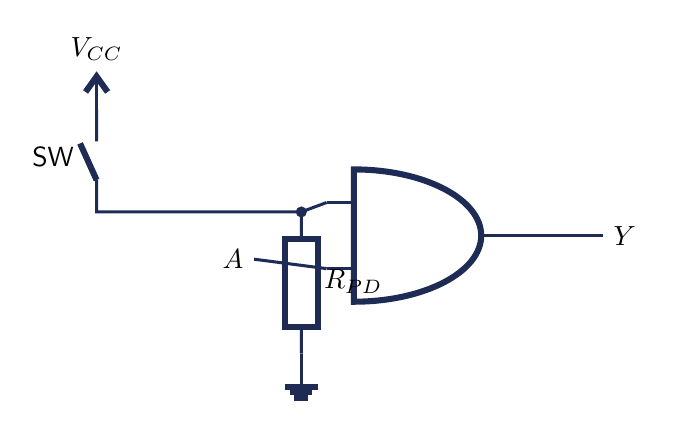
\begin{tikzpicture}[line width=1.1pt,draw=TEJNavy]
\node[and port,number inputs=2,scale=1.5] (gate) at (6.2,2.2) {};
\draw (3.8,2.5) -- (gate.in 1);
\draw (3.8,2.5) to[R,l=$R_{PD}$] (3.8,0.7) node[ground] {};
\draw (3.8,2.5) -- (1.2,2.5) to[nos,l=SW] (1.2,3.8) node[vcc] {$V_{CC}$};
\draw (3.2,1.9) node[left] {$A$} -- (gate.in 2);
\draw (gate.out) -- ++(1.2,0) node[right] {$Y$};
\fill[TEJNavy] (3.8,2.5) circle (2pt);
\end{tikzpicture}\end{document}
